\chapter{Monetary Policy (Text Ch. 30)}

\section{Monetary policy objectives and framework}

\subsection{The objective: price stability}

The Bank of Canada Act (1934) directs the Bank to regulate credit and currency in the best
interests of the economic life of the nation: to protect the external value of the
currency, to mitigate fluctuations in production, trade, prices and employment, and to
promote economic and financial welfare. In practice this has been interpreted as
\emph{price stability} as the primary goal, because a low and predictable inflation rate
is the best contribution monetary policy can make to sustained growth and employment.

\begin{definition}[Inflation-control target]
Since 1991 the Government of Canada and the Bank of Canada have agreed on an
\emph{inflation-control target}: to keep CPI inflation at \textbf{2\% a year}, the midpoint
of a \textbf{1\% to 3\%} control range. The agreement is renewed every five years (it was
renewed in 2016 and in 2021; the 2021 renewal kept the 2\% target while noting that the
Bank would also consider maximum sustainable employment).
\end{definition}

The Bank watches \emph{core inflation} measures (CPI-trim, CPI-median and CPI-common since
2016) to judge the underlying trend, because headline CPI is volatile (gasoline, food).

\begin{remark}[Why target inflation?]
\begin{itemize}
  \item An explicit target anchors \emph{inflation expectations}: wage and price
        setters expect about 2\%, which makes the target easier to hit.
  \item It provides accountability: the Bank must explain deviations.
  \item In the long run, monetary policy affects only the price level (the quantity
        theory), not potential GDP, so price stability is the goal it can actually achieve.
\end{itemize}
Since the mid-1990s Canadian CPI inflation has averaged close to 2\%, and it was mostly
inside the 1--3\% range until the post-pandemic surge in 2021.
\end{remark}

\subsection{Responsibility for monetary policy}

The \emph{Governing Council} of the Bank (the Governor, the Senior Deputy Governor and
the Deputy Governors) makes monetary policy decisions. Governors in this period were
Stephen Poloz (2013--2020) and Tiff Macklem (from 2020). The Bank is operationally
independent, but the government has ultimate responsibility: the Minister of Finance can
issue a written directive to the Bank (this has never been done), and the inflation target
is set jointly.

\section{The conduct of monetary policy}

\subsection{Choosing a policy instrument}

The Bank could target the monetary base, the exchange rate or a short-term interest rate.
It chooses an interest rate.

\begin{definition}[Overnight rate]
The \emph{overnight loans rate} is the interest rate on overnight loans that the big banks
make to each other. The Bank of Canada's monetary policy instrument is the
\emph{target for the overnight rate}.
\end{definition}

The Bank announces its overnight rate target on \textbf{eight fixed dates} each year
(introduced in 2000), four of which coincide with the quarterly \emph{Monetary Policy
Report}. Rate changes are usually in steps of 0.25 percentage points.

\subsection{Hitting the overnight rate target}

The Bank creates an \emph{operating band} 0.50 percentage points wide, centred on the
target:
\begin{itemize}
  \item the \textbf{bank rate} (top of the band, target $+ 0.25$) is the rate at which the
        Bank stands ready to lend reserves to banks. No bank would borrow from another bank
        at more than this rate;
  \item the \textbf{settlement balances rate} (bottom of the band, target $- 0.25$) is the
        rate the Bank pays on banks' deposits (settlement balances) at the Bank. No bank
        would lend to another at less than this.
\end{itemize}
So the overnight rate stays inside the band. Within the band, the Bank uses \emph{open
market operations} (buying or selling government securities, often as short-term
repurchase agreements) to adjust the quantity of settlement balances and keep the rate at
target.

\begin{example}
The target is 1.75\%, so the band is 1.50\% to 2.00\%: bank rate 2.00\%, settlement
balances rate 1.50\%. If the overnight rate starts to drift up to 1.85\% because banks
are short of reserves, the Bank buys securities (supplying reserves) until the rate is
back at 1.75\%. In March 2020 the Bank cut the target in three steps from 1.75\% to
0.25\%, which it called its \emph{effective lower bound}.
\end{example}

\subsection{The policy decision}

The Bank decides by forecasting inflation about 6 to 8 quarters ahead (because policy acts
with a lag). If projected inflation is above 2\% (or the economy has an inflationary
gap), it raises the overnight rate target; if projected inflation is below 2\% (a
recessionary gap), it cuts the target.

\begin{definition}[Taylor rule]
The \emph{Taylor rule} is a simple formula that summarizes how a central bank can set the
policy rate:
\[
  i = r^{*} + \pi + 0.5(\pi - \pi^{*}) + 0.5\,(\text{output gap}),
\]
where $r^{*}$ is the neutral real interest rate (often taken as 2\%), $\pi$ the inflation
rate, $\pi^{*}$ the target (2\%), and the output gap is in percent of potential GDP.
\end{definition}

\begin{example}
Inflation is 3\% and real GDP is 1\% above potential. Then
\[
  i = 2 + 3 + 0.5(3 - 2) + 0.5(1) = 6\%.
\]
If instead inflation is 1\% and the output gap is $-2\%$:
$i = 2 + 1 + 0.5(-1) + 0.5(-2) = 1.5\%$.
\end{example}

\begin{important}[Pitfall]
The Taylor rule raises the \emph{nominal} rate by \emph{more} than one-for-one with
inflation (by 1.5 points per point of inflation), so that the \emph{real} interest rate
rises when inflation rises. Raising the nominal rate by less than inflation would actually
ease policy.
\end{important}

\section{Monetary policy transmission}

A change in the overnight rate works its way through the economy in a series of steps.

\begin{center}
\begin{tikzpicture}[node distance=0.55cm, box/.style={draw, rounded corners, thick, align=center, minimum width=8.2cm, font=\small}]
  \node[box] (a) {Bank of Canada lowers the overnight rate target};
  \node[box, below=of a] (b) {Other short-term interest rates fall;\\ the Canadian dollar depreciates};
  \node[box, below=of b] (c) {Quantity of money and bank loans increase;\\ long-term real interest rate falls};
  \node[box, below=of c] (d) {Consumption, investment and net exports increase};
  \node[box, below=of d] (e) {Aggregate demand increases (multiplier)};
  \node[box, below=of e] (f) {Real GDP growth rises (about 1 year);\\ inflation rises (about 2 years)};
  \foreach \u/\v in {a/b, b/c, c/d, d/e, e/f} \draw[->, thick] (\u) -- (\v);
\end{tikzpicture}
\end{center}

\subsection{Step by step}

\begin{enumerate}
  \item \textbf{Interest rate changes.} When the overnight rate falls, other short-term
        rates (Treasury bill rates, banks' prime rate, variable mortgage rates) fall
        almost immediately. Long-term rates fall too, but by less, because they depend on
        expected future short-term rates.
  \item \textbf{Exchange rate.} A lower Canadian interest rate reduces the Canadian
        interest rate differential, so the demand for Canadian dollars decreases and the
        supply increases: the dollar depreciates.
  \item \textbf{Money and bank loans.} With cheaper reserves, banks expand loans and the
        quantity of money increases.
  \item \textbf{The long-term real interest rate} falls (if inflation expectations do not
        change much), which is what matters for spending decisions.
  \item \textbf{Expenditure plans.} Consumption increases (cheaper credit for cars and
        houses, higher asset prices), investment increases (more projects are profitable),
        and net exports increase (the depreciated dollar makes Canadian goods cheaper
        abroad and imports dearer).
  \item \textbf{Aggregate demand} increases by the multiplier times the change in
        expenditure.
  \item \textbf{Real GDP and inflation.} Real GDP growth and inflation rise. The Bank
        estimates that the full effect on output takes about 12 to 18 months and on
        inflation about 18 to 24 months.
\end{enumerate}
A rise in the overnight rate works the same way in reverse.

\subsection{Monetary policy to fight recession and inflation}

\begin{center}
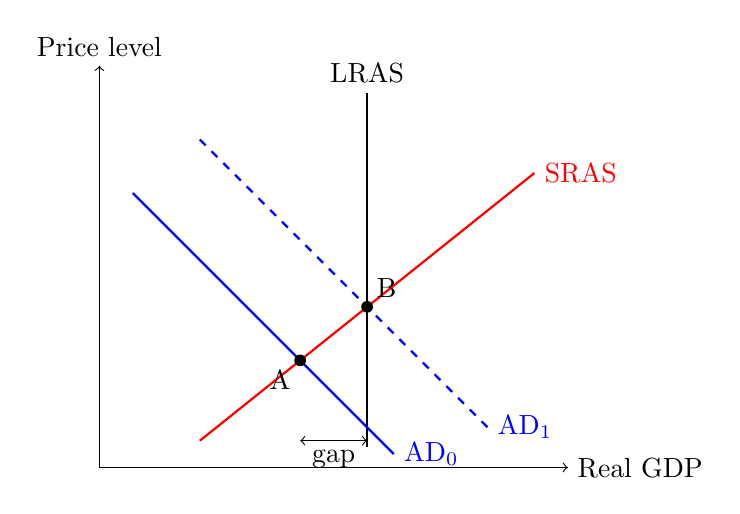
\begin{tikzpicture}[scale=0.85]
  \draw[->] (0,0) -- (7,0) node[right] {Real GDP};
  \draw[->] (0,0) -- (0,6) node[above] {Price level};
  \draw[thick] (4,0.3) -- (4,5.6) node[above] {LRAS};
  \draw[thick, red] (1.5,0.4) -- (6.5,4.4) node[right] {SRAS};
  \draw[thick, blue] (0.5,4.1) -- (4.4,0.2) node[right] {AD$_0$};
  \draw[thick, blue, dashed] (1.5,4.9) -- (5.8,0.6) node[right] {AD$_1$};
  \fill (3,1.6) circle (2.5pt) node[below left] {A};
  \fill (4,2.4) circle (2.5pt) node[above right] {B};
  \draw[<->] (3,0.4) -- node[below] {gap} (4,0.4);
\end{tikzpicture}
\end{center}

\begin{itemize}
  \item \textbf{Fighting recession (easing).} At A real GDP is below potential: a
        recessionary gap. The Bank lowers the overnight rate; through the transmission
        steps, AD shifts from AD$_0$ to AD$_1$ and the economy moves to B at potential GDP,
        with a somewhat higher price level.
  \item \textbf{Fighting inflation (tightening).} With an inflationary gap, the Bank raises
        the overnight rate: interest rates rise, the dollar appreciates, money and loans
        grow more slowly, spending falls and AD shifts leftward, closing the gap and
        bringing inflation down toward 2\%.
\end{itemize}

\subsection{Loose links and long and variable lags}

Monetary policy is hard because the links in the chain are loose:
\begin{itemize}
  \item \textbf{Long-term rates} may not move with the overnight rate (they depend on
        expected inflation and world rates; Canada is a small open economy).
  \item The \textbf{long-term real rate} depends on inflation expectations, which may
        change.
  \item \textbf{Expenditure plans} respond to many other factors (expected profits,
        confidence, the world economy), so the response to a given rate change varies.
  \item \textbf{Time lags} are long and variable, so the Bank must act on forecasts that
        can be wrong.
\end{itemize}

\begin{important}[Pitfall]
The Bank of Canada does not directly set mortgage rates, long-term bond yields or the
exchange rate. It sets the overnight rate target; everything else responds through
markets, often imperfectly.
\end{important}

\section{Extraordinary monetary policy}

When the overnight rate reaches its \emph{effective lower bound} (0.25\% in Canada in
2009--2010 and 2020--2022), the Bank cannot stimulate further by cutting it. In the
2008--2009 financial crisis and the 2020 pandemic it used other tools:
\begin{itemize}
  \item \textbf{Forward guidance}: a commitment to keep the rate low for an extended
        period (in 2009 a conditional commitment until mid-2010; in 2020 until the
        economy's slack was absorbed), lowering expected future short rates and so
        long-term rates.
  \item \textbf{Quantitative easing} (QE): large-scale purchases of Government of Canada
        bonds (begun in March 2020) to increase the monetary base and lower long-term
        interest rates.
  \item \textbf{Liquidity and credit facilities}: expanded lending to financial
        institutions against a wide range of collateral, and purchases of provincial,
        corporate and mortgage-backed assets to keep credit markets working.
\end{itemize}

\section{Comparing monetary and fiscal policy}

\begin{center}
\begin{tabular}{lll}
\toprule
 & Monetary policy & Fiscal policy \\
\midrule
Decided by & Bank of Canada & Government and Parliament \\
Main instrument & overnight rate target & spending, taxes, transfers \\
Decision lag & short (8 dates a year) & long (budget process) \\
Impact lag & 1--2 years & varies; can be fast for transfers \\
Main long-run effect & price level & potential GDP (supply side), debt \\
\bottomrule
\end{tabular}
\end{center}

\section{Summary}

\begin{itemize}
  \item The Bank of Canada's objective is price stability, made concrete as a 2\% inflation
        target (1--3\% range), renewed every five years.
  \item The instrument is the overnight rate target, announced on eight fixed dates; the
        operating band (bank rate on top, settlement balances rate at the bottom) and open
        market operations keep the overnight rate at target.
  \item The Taylor rule summarizes the policy response to inflation and the output gap.
  \item Transmission: overnight rate $\to$ other interest rates and exchange rate $\to$
        money and loans $\to$ long-term real rate $\to$ $C$, $I$, $NX$ $\to$ AD $\to$ real
        GDP (about 1 year) and inflation (about 2 years).
  \item Easing fights a recessionary gap; tightening fights inflation. Links are loose and
        lags long and variable.
  \item At the effective lower bound the Bank uses forward guidance, quantitative easing
        and credit facilities.
\end{itemize}
